%\section{Data}

\subsection{Imaging dataset}
%\item intro to M83: global parameters (distance, size, environment)
The dataset used for this study is the Wide-Field Camera-3
Early Release Science (ERS) observations of the nearby spiral galaxy Messier 83 (M83).
M83 is a grand-design spiral of type SAB, located at a distance of 4.66~Mpc \citep{tully13}
and the largest member of the M83 subgroup of the nearby Centaurus group of galaxies \citep{tully15}.
The galaxy's apparent radius of $\sim12$~arcmin \citep{} is reasonably well-matched to the camera's field of view.
{\bf And here we note some other interesting things about M83.}

%\item Intro to WFC3 ERS dataset
%\item existing studies with this dataset (cluster, massive stars, etc)
% ref: chandar10, section. TODO: check for (unintentional!) plagiarism
The objective of the ERS observations as a whole was to probe star formation in galaxies.
The observations of M83 were made in broad- and narrow-band filters in order to characterize both stellar and nebular properties.
They cover a $3.6\times3.6$~kpc$^2$ region in the northern portion of the galaxy, including the nucleus,
a portion of a spiral arm and an interarm region.
The spatial resolution of the images is $0\farcs0396$~arcsec~pixel$^{-1}$,
corresponding to a linear scale of $XX$~pc~pixel$^{-1}$ at the 4.66~Mpc distance.
A complete description of the observations and data processing is given by \citet{chandar10};
our work here uses the observations in the UVIS channel, listed in Table~\ref{tab:filters}.
A number of previous studies have used the ERS M83 dataset for various purposes.
These include studies of 
star clusters \citep{chandar10, wofford11, whitmore11, bastian11, bastian12, fouesneau12, silva13, andrews14, chandar14, adamo15,ryon15,hollyhead15, sun16},
H~{\sc ii} regions \citep{liu13}, supernova remnants and the interstellar medium \citep{dopita10, hong11, blair14, blair15}, 
resolved stars \citep{kim12, williams15},
and a super-Eddington off-nuclear black hole \citep{soria14}.


\begin{table}
\centering
\caption{\textbf{Need to fix ion function} List of filters from ERS survey with band names and exposure times.}
\label{tab:filters}
\begin{tabular}{lll}
\hline\hline
Filter & Name & Exposure time\\
\hline
F225W &  Wide UV & 1800~s\\
F336W &  $U$-band & 1890~s\\ 
%F373N &  [\ion{O}{iii}] & 2400~s\\
F438W &  $B$-band & 1180~s\\
F487N &  H$\beta$ & 2700~s\\
%F502N &  [\ion{O}{ii}] & 2484~s
F555W &  V-band, South field & 1203~s\\
%F547M &  V-band, North field & \\
%F657N &  H$\alpha$+[\ion{N}{ii}]& 1484~s\\ 
%F673N &  [\ion{S}{ii}] & 1850~s\\
F814W &  $I$-band & 1203~s\\
\hline
\end{tabular}
\end{table}

We analyze the catalog produced by \citet{chandar10} and made available via **REF**, hereafter referred to as the `ERS catalog.'
The objects in this catalog were detected on a `white-light' image produced by a weighted combination of the $UBVI$ images.
Photometry in 0.5- and 3-pixel radius apertures at the positions of the detected sources was performed on the broad- and narrow-band images and tabulated in the Vega magnitude system. 
We apply the correction to the F657N magnitude zeropoint (from 20.72 to 22.35) noted in the header of the catalog.
\citet{chandar10} discussed aperture corrections for this catalog, but since we are primarily concerned with colours
and the aperture correction does not vary strongly with wavelength, we omit it.
The catalog contains about 68000 objects which are expected to include individual stars, star clusters, stellar blends,
supernova remnants, H${\sc ii}$ regions, planetary nebulae, and background galaxies.
%TODO: foreground stars?
Completeness and reliability of the catalog are not discussed by \citet{chandar10},
but a visual inspection of the the detected sources on the white-light image suggests that a reasonable balance
between completeness and reliability was achieved.
Nine objects are flagged in the catalog as being problematic 
and we remove them from our analysis.

As a check on the catalog we used Sextractor to detect and photometer objects in the individual images.
While the aperture photometry measurements matched well, the derived uncertainties were much smaller than those reported in the catalog.
Indeed, the catalog uncertainties seem to be physically unreasonable, with median uncertainty values well above 1~magnitude in
most bandpasses, and the catalog notes do not recommend them for use except in a relative sense.
Our comparison implied that recovering a more typical magnitude uncertainty distribution would be accomplished by
dividing the 0.5-pixel magnitude uncertainties  by 10 for the broad-band filters and 15 for the narrow-band filters.
This allows us to use the catalog aperture magnitudes as an indicator of detected signal-to-noise: our analysis uses only objects with
(scaled) 0.5-pixel magnitude uncertainties $<0.2$~mag.
For the remainder of the analysis we use magnitudes measured in the 0.5-pixel radius aperture, as these should be less affected
by crowding and the variable galaxy background.

Table~\ref{tab:cat_numbers} and Figure~\ref{fig:mag_unc} characterize the catalog in terms of measurements in individual filters.
Not all objects are detected in all filters;
Table~\ref{tab:cat_numbers} gives the number of objects for which photometry is reported in a given filter,
the number for which scaled 0.5-pixel magnitude uncertainty is $0.2$~mag or less,
and the aperture magnitude at which the median magnitude uncertainty is $0.2$~mag. % Discuss last column and why 555 - should be because it is the broad filter with the most detections used for the whitelight image?
Figure~\ref{fig:mag_unc} shows the distributions of magnitudes and uncertainties in a broad and narrow filter. % See appendix for complete list of figures

%AK: please calculate numbers here. For the last column scipy.stats.binned_statistic is a good way to do this.
%Numbers are calculated based on the 0.5 aperture filters - can be changed if we decide otherwise
\begin{table}
\centering
\caption{List of filter names with the number of objects detected, the number of objects with an uncertainty < 0.2 mag, and the 0.5 px aperture magnitude for which the median uncertainty is 0.2.}
\label{tab:cat_numbers}
\begin{tabular}{lrrlr}
\hline\hline
Filter & $N_{\rm obj}$ & $N_{\rm good}$ & $m_{\rm good}$ \\
\hline
F225W &  57237 & 15011 & 25.159 \\
F336W &  62192 & 34129 & 26.574 \\
F373N &  55966 & 8878 & 24.752 \\
F438W &  66356 & 48858 & 28.048 \\
F487N &  63812 & 13335 & 25.77 \\
F502N &  64313 & 14654 & 26.424 \\
F555W &  67424 & 65652 & 30.059 \\
F657N &  67782 & 67634 & 26.855 \\
F673N &  65305 & 25295 & 26.284 \\
F814W &  67050 & 59600 & 27.8699 \\
\hline
\end{tabular}
\end{table}

%AK: here's where the plots go.
\begin{figure*}
\centering
\subfloat[Broad filter distribution.]{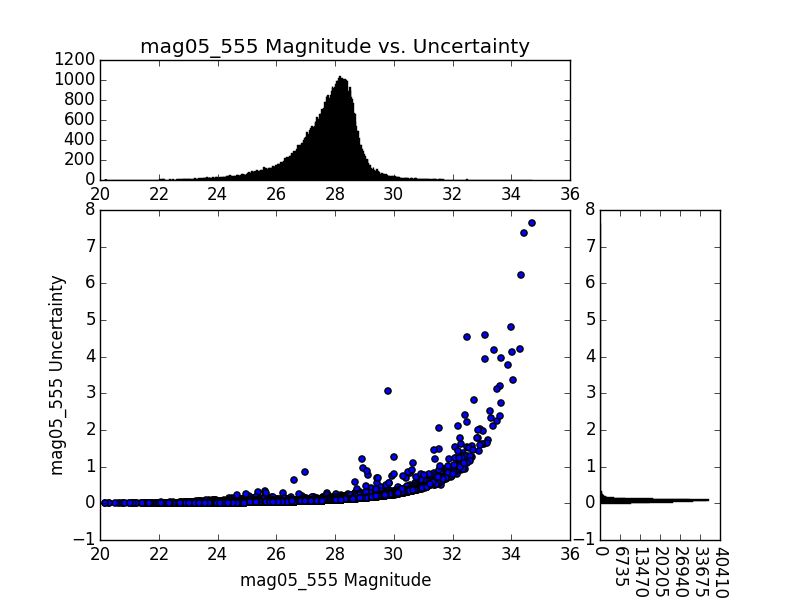
\includegraphics[width=0.5\textwidth]{figs/mag05_555_uncertainty_distribution}\label{fig:mag_unc_broad}}
\hfill
\subfloat[Narrow filter distribution.]{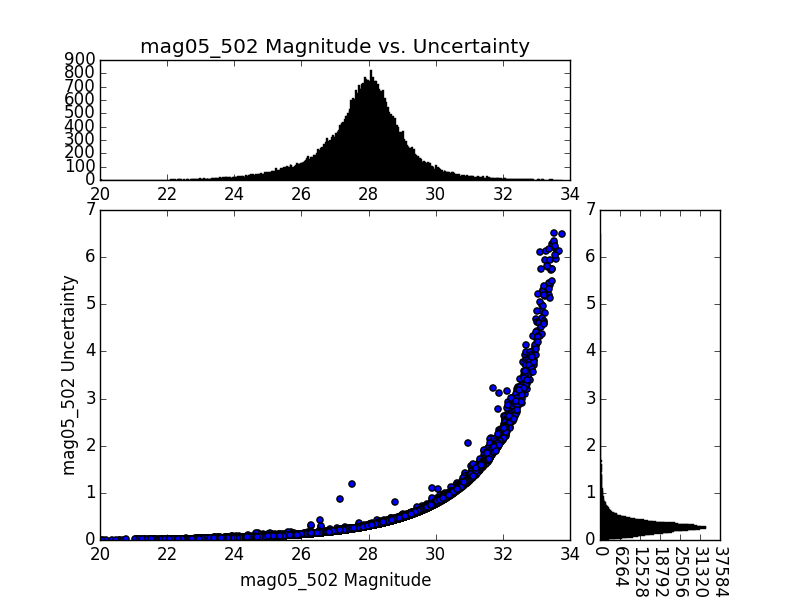
\includegraphics[width=0.5\textwidth]{figs/mag05_502_uncertainty_distribution}\label{fig:mag_unc_narrow}}
\caption{Distribution of magnitudes and uncertainties for objects in the \citet{chandar10} M83 ERS catalog.}
\label{fig:mag_unc}
\end{figure*}

\subsection{Colour Models}
\textbf{Discuss colour models. Figure is broad-band combination with model.}

\begin{figure}
\label{fig:model_colour}
\centering
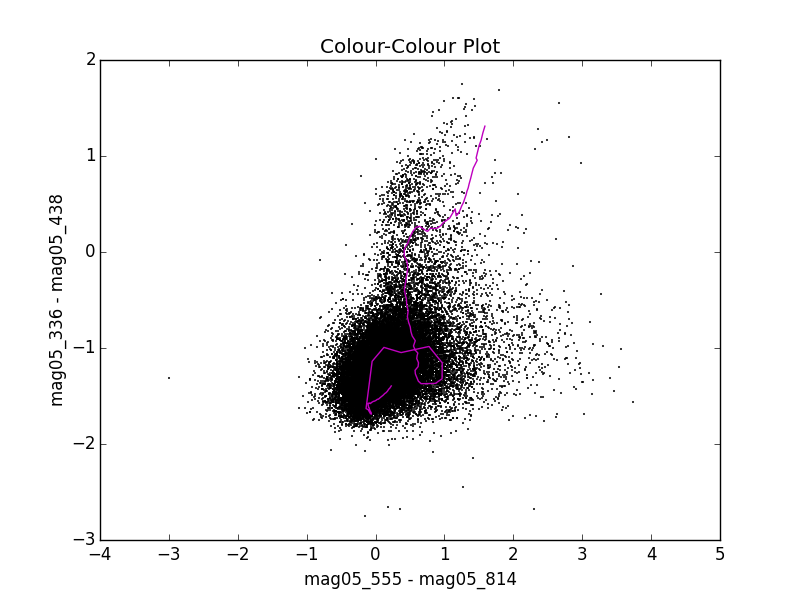
\includegraphics[width=0.5\textwidth]{figs/data/plot_mag05_555-mag05_814vsmag05_336-mag05_438}
\caption{Colour-colour distribution of $V - I$ and $U - B$ with colour model plotted in pink.}
\end{figure}

%Outline for data section
%%\begin{enumerate}
%\item Intro to WFC3 ERS dataset
%\item intro to M83: global parameters (distance, size, environment)
%\item existing studies with this dataset (cluster, massive stars, etc)
%\item description of catalog (is there a ref for this??)
%\item anything about these data we don't like/didn't use?

%\end{enumerate}

